\documentclass[12pt,fleqn]{article}\usepackage{../../common}
\begin{document}
Sonlu Öğeler Metotu (Finite Elements Method -FEM-) - 2

Önceki örnekler standart eni değişmeyen kiriş yapısını temel aldı.  Fakat ya
kiriş alttaki gibi olsaydı?

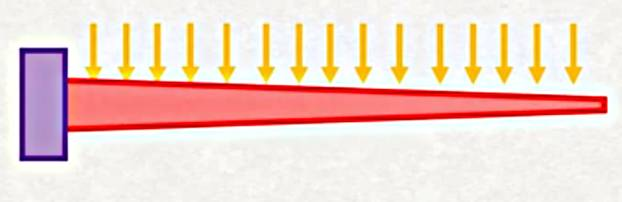
\includegraphics[width=20em]{compscieng_bpp45fem2_01.jpg}

Bu kirişi temsilen

$$
E I \frac{\ud^4 y}{\ud X_1^4} = q
$$

diferansiyel denklemini hala kullanabilir miyiz? Dikkat edersek en değiştiğine
göre $X_1$ ile beraber, ona bağlı olarak, atalet momenti $I$ sabit değil,
değişken demektir.. Bazıları düşünebilir ``ama o zaman değişken $I$'yi alırız,
üstteki denklemdeki $I$'ya sokarız olur biter''. Bunu yapamayız çünkü $I$'nin
sabit olması üstteki denklemi türetmek için bir önkabuldu, yani $I$ değişken ise
üstteki denklemi kullammak mümkün değildir.















\end{document}
